\documentclass[12pt]{article}

\usepackage{cmap}
\usepackage[T2A]{fontenc}
\usepackage[utf8]{inputenc}
\usepackage[russian]{babel}
\usepackage{graphicx}
\usepackage{amsthm,amsmath,amssymb}
\usepackage{listings}
\usepackage{color}
\usepackage[table]{xcolor}
\usepackage{colortbl}
\usepackage{array}
\usepackage{epigraph}
\usepackage{textcomp}

\usepackage[russian,colorlinks=true,urlcolor=red,linkcolor=blue]{hyperref}
\usepackage{enumerate}
\usepackage[shortlabels]{enumitem}
\usepackage{datetime}
\usepackage{fancyhdr}
\usepackage{lastpage}
\usepackage{verbatim}
\usepackage{tikz}
\usetikzlibrary{arrows,patterns,decorations.markings,decorations.pathmorphing,decorations.pathreplacing}
\usetikzlibrary{math,positioning}
\usepackage{pgfplots}

\usepackage{ifthen}
\usepackage{mathtools}
\usepackage{mdframed}
\usepackage[normalem]{ulem}

\graphicspath{ {notes-15-diffusion} }

\def\SEASON{2024/25}


\sloppy
\voffset=-20mm
\textheight=235mm
\hoffset=-22mm
\textwidth=180mm
\headsep=12pt
\footskip=20pt

\parskip=0em
\parindent=0em

\setlength\epigraphwidth{.8\textwidth}

\newlength{\tmplen}
\newlength{\tmpwidth}
\newlength{\storelen}
\newcounter{listcounter}

% Список с маленькими отступами
\newenvironment{MyList}[1][4pt]{
  \begin{enumerate}[1.]
  \setlength{\parskip}{0pt}
  \setlength{\itemsep}{#1}
}{       
  \end{enumerate}
}
% Вложенный список с маленькими отступами
\newenvironment{InnerMyList}[1][0pt]{
  \vspace*{-0.5em}
  \begin{enumerate}[(a)]
  \setlength{\parskip}{-0pt}
  \setlength{\itemsep}{#1}
}{       
  \end{enumerate}
  \vspace*{-0.5em}
}
% Список с маленькими отступами
\newenvironment{MyItemize}[1][4pt]{
  \begin{itemize}
  \setlength{\parskip}{0pt}
  \setlength{\itemsep}{#1}
}{       
  \end{itemize}
}

% Основные математические символы
\def\TODO{{\color{red}\bf TODO}}
\def\N{\mathbb{N}}       %
\def\R{\mathbb{R}}       %
\def\F2{\mathbb{F}_2}    %
\def\Z{\mathbb{Z}}       %
\def\H{\mathcal{H}}      % семество хеш-функций
\def\E{\mathsf{E}}       % матожидание
\def\INF{\infty}    % +inf
\def\EPS{\varepsilon}    %
\def\EMPTY{\varnothing}  %
\def\PHI{\varphi}        %
\def\SO{\Rightarrow}     % =>
\def\EQ{\Leftrightarrow} % <=>
\def\t{\texttt}          % mono font
\def\c#1{{\rm\sc{#1}}}   % font for classes NP, SAT, etc
\def\O{\mathcal{O}}      %
\def\NO{\t{\#}}          % #
\def\XOR{\text{ {\raisebox{-2pt}{\ensuremath{\Hat{}}}} }}
\def\xor{\t{\^{}}}
\renewcommand{\le}{\leqslant}
\renewcommand{\ge}{\geqslant}
\newcommand{\q}[1]{\langle #1 \rangle}               % <x>
\newcommand\URL[1]{{\footnotesize{\url{#1}}}}        %
\newcommand{\sfrac}[2]{{\scriptstyle\frac{#1}{#2}}}  % Очень маленькая дробь
\newcommand{\mfrac}[2]{{\textstyle\frac{#1}{#2}}}    % Небольшая дробь
\newcommand{\score}[1]{{\bf\color{red}{(#1)}}}
\newcommand{\divby}{\mathop{\raisebox{-2pt}{\vdots}}}

\newcommand{\fix}[1]{{\color{fixcolor}{#1}}} % \underline
\def\bonus{\t{\red{(*)}}}
\def\ifbonus#1{\ifthenelse{\equal{#1}{}}{}{\bonus}}
\def\smallsquare{$\scalebox{0.5}{$\square$}$}
\def\vstick{^\t{\textquotesingle}}
\def\bluebox#1{\fcolorbox{blue}{white}{#1}}

\newlength{\myItemLength}
\setlength{\myItemLength}{0.3em}
\def\ItemSymbol{\smallsquare}
\def\Item{\vspace*{\myItemLength}\ItemSymbol \ \ }

\newcommand{\LET}{%
  % [line width=0.6pt]
  \begin{tikzpicture}%
  \draw(0.8ex,0) -- (0.8ex,1.6ex);%
  \draw(0,1.6ex) -- (0.8ex,1.6ex);%
  \end{tikzpicture}%
  \hspace*{0.1em}%
}

% Отступы
\def\makeparindent{\hspace*{\parindent}\unskip}
\def\up{\vspace*{-0.5em}}%{\vspace*{-\baselineskip}}
\def\down{\vspace*{0.5em}}
\def\LINE{\vspace*{-1em}\noindent \underline{\hbox to 1\textwidth{{ } \hfil{ } \hfil{ } }}}
\def\BOX#1{\mbox{\fbox{\bf{#1}}}}
\def\Pagebreak{\pagebreak\vspace*{-1.5em}}
\def\RIGHT{\hspace*{\fill}} % сдвинуться до упора вправо
\def\NewLine{\hspace*{1em}\\}

% Мелкий заголовок
\newcommand{\THEE}[1]{
  \vspace*{0.5em}
  \noindent{\bf \underline{#1}}%\hspace{0.5em}
  \vspace*{0.2em}
}
% Другой тип мелкого заголовка
\newcommand{\THE}[1]{
  \vspace*{0.5em} $\bullet$
  \noindent{\bf #1}%\hspace{0.5em}
  \vspace*{0.2em}
}

\newenvironment{MyTabbing}{
  \t\bgroup
  \vspace*{-\baselineskip}
  \begin{tabbing}
    aaaa\=aaaa\=aaaa\=aaaa\=aaaa\=aaaa\kill
}{
  \end{tabbing}
  \t\egroup
}

% Код с правильными отступами
\lstnewenvironment{code}{
  \lstset{}
%  \vspace*{-0.2em}
}%
{
%  \vspace*{-0.2em}
}
\lstnewenvironment{codep}{
  \lstset{language=python}
}%
{
}
% Код, содержащий выскоие формулы, вставить не так просто...
\def\codeinput#1{
  \begin{mdframed}[innertopmargin=-2pt,innerbottommargin=-2pt,innerleftmargin=4pt,backgroundcolor=lightgray]
  \lstinputlisting[frame={}]{#1}
  \end{mdframed}
}

% Формулы с правильными отступами
\newenvironment{smallformula}{
 
  \vspace*{-0.8em}
}{
  \vspace*{-1.2em}
  
}
\newenvironment{formula}{
 
  \vspace*{-0.4em}
}{
  \vspace*{-0.6em}
  
}

% Большая квадратная скобка
\makeatletter
\newenvironment{sqcases}{%
  \matrix@check\sqcases\env@sqcases
}{%
  \endarray\right.%
}
\def\env@sqcases{%
  \let\@ifnextchar\new@ifnextchar
  \left\lbrack
  \def\arraystretch{1.2}%
  \array{@{}l@{\quad}l@{}}%
}
\makeatother

% Определяем основные секции: \begin{Lm}, \begin{Thm}, \begin{Def}, \begin{Rem}
\renewcommand{\qedsymbol}{$\blacksquare$}
\theoremstyle{definition} % жирный заголовок, плоский текст
\newtheorem{Thm}{Th}[subsection] % нумерация будет "<номер subsection>.<номер теоремы>"
\newtheorem{Lm}[Thm]{Lm} % Нумерация такая же, как и у теорем
\newtheorem{Ex}[Thm]{Упражнение} % Нумерация такая же, как и у теорем
\newtheorem{Example}[Thm]{Пример} % Нумерация такая же, как и у теорем
\newtheorem{Code}[Thm]{Код} % Нумерация такая же, как и у теорем
\theoremstyle{plain} % жирный заголовок, курсивный текст
\newtheorem{Def}[Thm]{Def} % Нумерация такая же, как и у теорем
\newtheorem{Algo}[Thm]{Алгоритм} % Нумерация такая же, как и у теорем
\theoremstyle{remark} % курсивный заголовок, плоский текст
\newtheorem{Cons}[Thm]{Следствие} % Нумерация такая же, как и у теорем
\newtheorem{Conj}[Thm]{Гипотеза} % Нумерация такая же, как и у теорем
\newtheorem{Prop}[Thm]{Утверждение} % Нумерация такая же, как и у теорем
\newtheorem{Rem}[Thm]{Замечание} % Нумерация такая же, как и у теорем
\newtheorem{Remark}[Thm]{Замечание} % Нумерация такая же, как и у теорем
\newtheorem{Img}[Thm]{Иллюстрация} % Нумерация такая же, как и у теорем

\def\SectionName{Название секции}
\def\AuthorName{Тихонов Даниил}

\newlength{\sectionvskip}
\setlength{\sectionvskip}{0.5em}
\newcommand{\Section}[5][]{
  % Заголовок
  \pagebreak
%  \ifthenelse{\isempty{#1}}{
    \refstepcounter{section}
%  }{}
  \vspace{0.5em}
%  \ifthenelse{\isempty{#1}}{
%    \addtocontents{toc}{\protect\addvspace{-5pt}}%
    \addcontentsline{toc}{section}{\arabic{section}. #2}
%  }{}
  \begin{center}
    {\Large \bf Лекция \NO{#4}: #2} \\ 
    \vspace{\sectionvskip}
    \ifthenelse{\equal{#3}{}}{}{{\large #3}\\}
    % {\large #3} \\
  \end{center}

  \LINE

  % Запомнили название и автора главы
  \gdef\SectionName{#2}
  \gdef\AuthorName{#4}

  % Заголовок страницы
  \lhead{Глубинное обучение 1, \SEASON}
  \chead{}
  \rhead{ФКН ВШЭ}
  \renewcommand{\headrulewidth}{0.4pt}

  \lfoot{Лекция \NO{#4}. #3.}
  \cfoot{\thepage\t{/}\pageref*{LastPage}}
  \rfoot{Лектор: Шипилов Фома}
  \renewcommand{\footrulewidth}{0.4pt}
}

\newcommand{\Subsection}[2][]{
  \refstepcounter{subsection}
  \vspace*{1em}
  \ifthenelse{\equal{#1}{}}
    {\addcontentsline{toc}{subsection}{\arabic{section}.\arabic{subsection}. #2}}
    {\addcontentsline{toc}{subsection}{\arabic{section}.\arabic{subsection}. \bonus\,#2}}
  {\color{blue}\bf\large \arabic{section}.\arabic{subsection}. \ifbonus{#1}\,{#2}} 
  \vspace*{0.5em}
  \makeparindent
}
\newcommand{\Subsubsection}[2][]{
  \refstepcounter{subsubsection}
  \vspace*{1em}
  \ifthenelse{\equal{#1}{}}
    {\addcontentsline{toc}{subsubsection}{\arabic{section}.\arabic{subsection}.\arabic{subsubsection}. #2}}
    {\addcontentsline{toc}{subsubsection}{\arabic{section}.\arabic{subsection}.\arabic{subsubsection}. \bonus\,#2}}
  {\color{blue}\bf\large \arabic{section}.\arabic{subsection}.\arabic{subsubsection}. \ifbonus{#1}\,#2}
  \vspace*{0.5em}
  \makeparindent
}

\newcommand{\Header}{
  \pagestyle{empty}
  \renewcommand{\dateseparator}{--}
  \begin{center}
    {\Large\bf 
     ФКН ВШЭ\\
     %Первый курс, \SEASON\\
    \vspace{0.3em}
    Глубинное обучение 1, \SEASON}\\
    \vspace{0.7em}
    Автор конспекта: Даниил Тихонов \\
    \vspace{0.7em}
    {{\today} в {\currenttime}}
  \end{center}

  \LINE
  \vspace{0em}

  \renewcommand{\baselinestretch}{0.98}\normalsize
  \tableofcontents
  \renewcommand{\baselinestretch}{1.0}\normalsize
  \pagebreak
}

\newcommand{\BeginConspect}{
  \pagestyle{fancy}
  \setcounter{page}{1}
}

\def\Bibliography#1#2#3{\href{#1}{\t{[#2]}}. #3}
\def\Link#1#2#3{\href{#1}{\t{[#2]}}. #3}
\def\ShortLink#1#2{\href{#2}{\t{[#1]}}}

\definecolor{mygray}{rgb}{0.7,0.7,0.7}
\definecolor{ltgray}{rgb}{0.9,0.9,0.9}
\definecolor{fixcolor}{rgb}{0.7,0,0}
\definecolor{red2}{rgb}{0.7,0,0}
\definecolor{dkred}{rgb}{0.4,0,0}
\definecolor{dkblue}{rgb}{0,0,0.6}
\definecolor{dkgreen}{rgb}{0,0.6,0}
\definecolor{brown}{rgb}{0.5,0.5,0}

\newcommand{\green}[1]{{\color{green}{#1}}}
\newcommand{\black}[1]{{\color{black}{#1}}}
\newcommand{\red}[1]{{\color{red}{#1}}}
\newcommand{\dkred}[1]{{\color{dkred}{#1}}}
\newcommand{\blue}[1]{{\color{blue}{#1}}}
\newcommand{\dkgreen}[1]{{\color{dkgreen}{#1}}}


\setlength\parindent{20pt} 

\begin{document}

\Header
\BeginConspect

\Section{Диффузионные модели}{3 марта, 2025}{15}

\Subsection{Denoising Diffusion Probabilistic Models (DDPM)}

    Если в самых общих словах описывать диффузионные модели, то идея следующая: возьмем какую-то картинку и будем постепенно на каждом шаге добавлять в нее стандартный нормальный шум, пока она полностью не превратится в шум. Затем обучим модель, которая, наоборот, будет убирать из нее немного шума на каждом шаге, пока не получится картинка. \\

    Предположим, что наши данные являются векторами $x \in \R^n$. Теперь для каждого момента времени $t \in [0, \,T] \cap \mathbb{Z}$ зададим вероятностное распределение на $x$ таким образом, что
    \begin{itemize}
        \item $x_0 \sim p_{data}$, где $p_{data}$ -- распределение реальных данных
        \item $x_T \sim \mathcal{N}(0, \, I)$
        \item $q(x_t \, | \, x_{t-1}) := \mathcal{N}\left(\sqrt{1-\beta_t} \, x_{t-1}, \, \beta_t \, I\right)$, где $\beta_t$ -- это какое-то маленькое число, зависящее от времени $t$ (в простейшем случае можно думать, что $\beta_t \equiv \beta$ -- константа).
    \end{itemize}

    В данной модели $q(x_t \, | \, x_{t-1})$ задает некоторый марковский процесс или же правило, по которому данные переводятся в шум в каждый момент времени $t$.

    \begin{center}
    \fbox{\begin{minipage}{0.79\textwidth}
    \[
    \text{Задаваемый }\textcolor{teal}{q(x_t \, | \, x_{t-1})} \text{ процесс называется} \textbf{ прямым процессом}.
    \]
    
    \end{minipage}} 
    \end{center}

    Запишем совместное распределение всей траектории:
    \[
    q(x_{1:T} \, | \, x_0) := q(x_1, \dots, x_T \, | x_0) = \prod_{t=1}^T q(x_t \, | x_{t-1})
    \]

    То есть пока все достаточно просто: картинка зашумляется, информация из нее исчезает, энтропия увеличивается. Нейросеть мы будем учить разворачивать этот прямой процесс, то есть получать на вход шум $z \in \mathcal{N}(0, \, I)$ и делать обратные шаги (расшумлять картинку). \\

    \begin{center}
        \begin{tabular}{cc}
            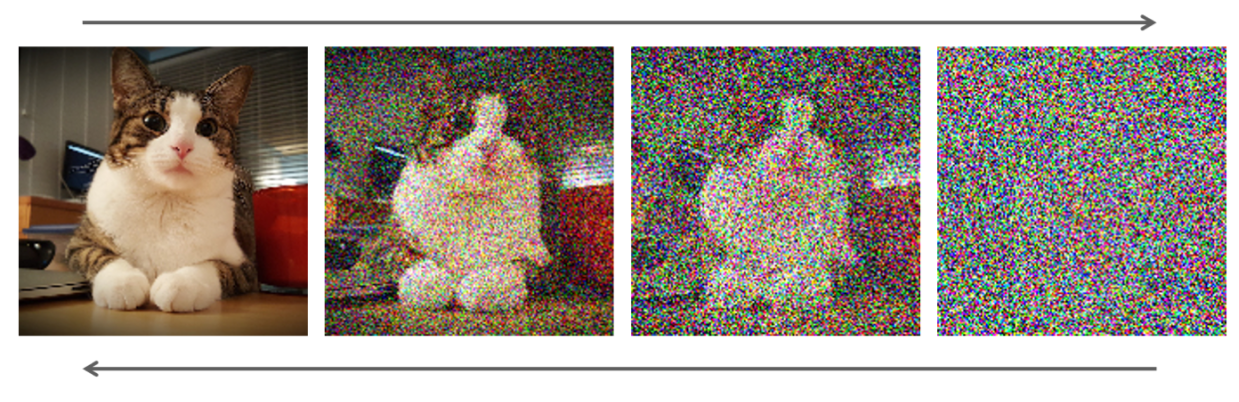
\includegraphics[scale=0.50]{Снимок.PNG}
        \end{tabular}
    \end{center}

    \pagebreak

    Зададим эту модель с параметрами $\theta$ следующим образом:
    \[
    p_\theta(x_{t-1} \, | \, x_t) := \mathcal{N}\left(x_{t-1}\, | \,\mu_\theta(x_t, \, t), \,\Sigma_\theta(x_t, \, t)\right)
    \]

    На самом деле, в общем случае матрицу ковариации можно не обучать, и просто полагать
    \[
    p_\theta(x_{t-1} \, | \, x_t) := \mathcal{N}\left(x_{t-1} \, | \, \mu_\theta(x_t, \, t), \, \textcolor{red}{\beta_t \, I}\right)
    \]

    В таком сетапе совместное распределение всей траектории имеет вид:
    \[
    p_\theta(x_{0:T}) := p_\theta(x_0, \dots, x_T) = p(x_T) \,\prod_{t=1}^Tp_\theta(x_{t-1} \, | \, x_t), \quad p(x_T) \sim \mathcal{N}(0, \, I)
    \]

    Предположим, что мы уже справились обучить модель $p_\theta$. Тогда ниже представлен алгоритм семплирования из нее новых данных:
        \begin{itemize}
            \item Семплируем $x_T \sim \mathcal{N}(0, \, I)$
            \item Для каждого $t = 1, \dots, T$ семплируем $x_{t-1} \sim p_\theta(x_{t-1} \, | \, x_t)$
            \item Получаем сгенерированный объект $x_0$
        \end{itemize}

    Заметим, что на каждом шаге семплирования из пункта $(2)$ картинка постепенно расшумляется, но при этом в нее все равно добавляется немного шума из-за дисперсии $\textcolor{red}{\beta_t \, I}$. \\

        Конечной целью является возможность семплировать из распределения данных, то есть
        \[
        x_0 \sim p_{data}
        \]
        
        Поэтому учить модель мы будем, максимизируя правдоподобие сгенерированного объекта:
        \[
        \log p_\theta(x_0) = \log \int  p_\theta(x_{0:T}) \, dx_1 \dots dx_T = 
        \log \int  \textcolor{blue}{q(x_{1:T} \, | \, x_0)} \, \frac{p_\theta(x_{0:T})}{\textcolor{blue}{q(x_{1:T} \, | \, x_0)}} \, dx_1 \dots dx_T =
        \]
        
        \[
        = \log \mathbb{E}_{\textcolor{black}{q(x_{1:T} \, | \, x_0)}} \bigg[\frac{p_\theta(x_{0:T})}{\textcolor{black}{q(x_{1:T} \, | \, x_0)}}\bigg] \,\textcolor{red}{\geq} \, \mathbb{E}_{\textcolor{black}{q(x_{1:T} \, | \, x_0)}} \bigg[\log \frac{p_\theta(x_{0:T})}{\textcolor{black}{q(x_{1:T} \, | \, x_0)}}\bigg] \longrightarrow \max_{\theta}
        \]\\
        
        В \textcolor{red}{переходе выше} мы воспользовались неравенством Йенсена для логарифма. Как и во многих других моделях, будем максимизировать нижнюю оценку, таким образом косвенно максимизируя исходное правдоподобие. Распишем нижнюю оценку, используя формулы выше:
        \[
        \mathbb{E}_{\textcolor{black}{q(x_{1:T} \, | \, x_0)}} \bigg[\log \frac{p_\theta(x_{0:T})}{\textcolor{black}{q(x_{1:T} \, | \, x_0)}}\bigg] = \mathbb{E}_{q(x_{1:T} \, | \, x_0)} \bigg[ \frac{p(x_T) \,\prod_{t=1}^Tp_\theta(x_{t-1} \, | \, x_t)}{\prod_{t=1}^T q(x_t \, | x_{t-1})}\bigg] =
        \]
        \[
        = \mathbb{E}_{\textcolor{black}{q(x_{1:T} \, | \, x_0)}} \bigg[\log p(x_T) + \sum_{t=1}^T\frac{p_\theta(x_{t-1} \, | \, x_t)}{q(x_t \, | x_{t-1})} \bigg] =: \mathcal{L}\textit{oss}
        \]

        \pagebreak

        В явном виде этот интеграл считать трудно, так как матожидание берется по какому-то сложному распределению. Вместо этого будет приближать лосс методом Монте-Карло:

        \begin{itemize}
            \item Берем обучающий объект $x_0$ из датасета
            \item Семплируем для него траекторию прямого процесса $x_1 \sim q(x_1 \, | \, x_0), \dots, x_T \sim q(x_T \, | \, x_{T-1})$
            \item Считаем $\nabla_\theta \, \left(\sum_{t=1}^T\frac{p_\theta(x_{t-1} \, | \, x_t)}{q(x_t \, | x_{t-1})}\right)$ и обновляем параметры $\theta$
        \end{itemize}

        В такой постановке возникает проблема, что для одного шага градиентного спуска нужно семплировать всю траекторию (сгенерировать $T$ картинок), что очень долго. \\

        На практике матожидание из лосса на самом деле можно уточнить:
        \[
        \mathbb{E}_{q(x_{1:T} \, | \, x_0)}\bigg[ -\text{KL}\left(\textcolor{red}{q(x_T \, | \, x_1)}\,\, \big|\big| \,\, p(x_T)\right) - \sum_{t=1}^T\text{KL}\left(\textcolor{blue}{q(x_{t-1} \, | \, x_t,\, x_0)}\,\, \big|\big| \,\, p_\theta(x_{t-1} \, | \, x_t)\right) + \log p_\theta(x_0 \, | \, x_1) \bigg]
        \]

        Смотря на эту формулу вряд ли можно подумать, что стало легче. Но заметим, что
        \[
        \textcolor{blue}{q(x_{t-1} \, | \, x_t,\, x_0)} = \frac{q(x_{t-1}, \, x_t,\, x_0)}{q(x_t,\, x_0)} = \frac{q(x_0) \, q(x_{t-1} \, | \, x_0) \, q(x_t \, | \, x_{t-1})}{q(x_0) \, q(x_t \, | x_0)} = \frac{q(x_{t-1} \, | \, x_0) \, q(x_t \, | \, x_{t-1})}{q(x_t \, | x_0)}
        \]

        Все распределения в оставшейся формуле являются нормальными из пространства одной размерности. Исходя из вида плотности многомерного нормально распределения можно понять, что $q(x_{t-1} \, | \, x_t,\, x_0)$ тоже является нормальным распределением. \\

        В новой формуле также появилось интересное распределение $\textcolor{red}{q(x_T \, | \, x_1)}$, которое отвечает за семплирование на целых $T$ шагов вперед, хотя до этого мы семплировали от предыдущего шага к следующему. \\
        
        Из того, как был введен марковский процесс, можно понять, что семплирование на несколько шагов вперед будет суммой случайных нормальных векторов:
        \[
        {q(x_t \, | \, x_1)} = \mathcal{N}\left(x_t \, \bigg| \, \prod_{i=1}^t\sqrt{1 - \beta_i} \, x_0, \, \left(1 - \prod_{i=1}^t\beta_i\right)I\right)
        \]

        Поэтому $\textcolor{red}{q(x_T \, | \, x_1)}$ тоже является нормальным распределением. \\

        Возвращаясь к вопросу о простоте новой формулы лосса, все распределения в KL-дивиргенциях оказываются нормальными, а для их вычисления известна аналитическая формула, поэтому проблем при подсчете не возникнет. \\

        Зато можно показать, что засчет того, что в новой оценке часть матожидания уже вычислена, у нее будет меньше дисперсия. Более того, теперь нет необходимости семплировать всю траекторию для обучения.

        \pagebreak

        Действительно, засчет возможности семплирования на несколько шагов вперед, можно вместо всей траектории брать случайные моменты. Новый алгоритм обучения описывается так:
        \begin{itemize}
            \item Семплируем момент времени $t \sim U[1, \dots, T]$ и $x_t \sim q(x_t \, | \, x_0)$
            \item Считаем градиент и обновляем параметры $\theta$:
            \[
            \nabla_\theta \, \left(\text{KL}\left(\textcolor{black}{q(x_{t-1} \, | \, x_t,\, x_0)}\,\, \big|\big| \,\, p_\theta(x_{t-1} \, | \, x_t)\right)\right)
            \]
        \end{itemize}

        Таким образом, получили сильно более эффективное обучение. Однако при этом генерация все равно будет работать в $T$ шагов, что ощутимо медленнее, чем в тех же GANах. \\

        Для того, чтобы ускорить именно инференс, нужно перейти в непрерывное время.

    \Subsection{Обыкновенные дифференциальные уравнения}

    Введем $x_t \in \R^n$, время $t \in [0, \, T]$ и направление $dx_t$, которое в каждый момент времени выражается через векторное поле, а также начальное условие. Более формально:
    \[
    \begin{cases}
        dx_t = f(x_t, \, t)  \, dt \\
        x_0 = v \in \R^n
    \end{cases}
    \]

    Такое уравнение задает некоторую траекторию $x_t$ до момента времени $T$: 

    \begin{center}
        \begin{tabular}{cc}
            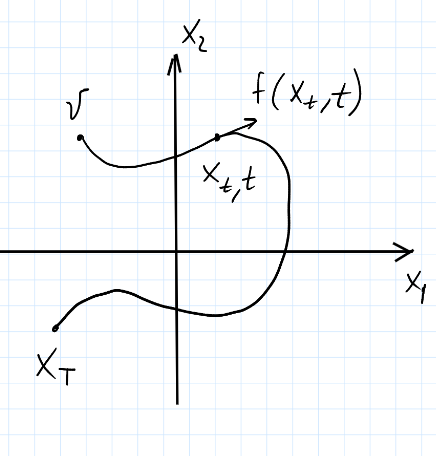
\includegraphics[scale=0.70]{Снимок2 (2).PNG}
        \end{tabular}
    \end{center}

    Используя схему интегрирования Эйлера, можно численно посчитать для любого начального условия $v$ всю траекторию $x_t$ до момента времени $T$:
    \[
    x_{t+h} = x_t + hf(x_t, \, t) + o(h) \approx x_t + hf(x_t, \, t)
    \]

    \pagebreak

    Хочется описывать диффузию с непрерывным временем как непрерывную траекторию, которая из картинки переходит в шум. К сожалению, одних обыкновенных дифференциальных уравнений для этого не хватает, так как в диффузии траектории на самом деле случайные.

    \Subsection{Стохастические дифференциальные уравнения}

    Для этого будем работать со стохастическими дифференциальными уравнениями, которые преобразовывают во времени не сам $x_t$, а его распределение (распределение траекторий). \\

    Формальная постановка очень похожа на предыдущую:
    \[
    \begin{cases}
        dx_t = f(x_t, \, t) \, dt \, \textcolor{red}{+g(t) \, dW_t} \\
        x_0 \sim p_0 \text{ -- начальное распределение}
    \end{cases}
    \]
    
    То есть в отличие от прошлой постановки, в каждый момент времени $x_t$ дополнительно движется в случайном направлении $dW_t$, где $W_t$ -- стандартный винеровский процесс. \\

    С помощью той же схемы интегрирования Эйлера, получаем
    \[
    x_{t+h} \approx x_t + hf(x_t, \, t) + \sqrt{h} \,g(t) \, \varepsilon_t, \quad \varepsilon_t \sim \mathcal{N}(0, \, I)
    \]

    Решением будет являться распределение на траектории $x_t \sim p_t$. \\

    \Subsection{Обращение времени}
    
    Процесс зашумления картинки на самом деле можно представить в виде стохастического уравнения выше, но нас интересует именно обратный процесс. \\
    
    Другими словами, мы хотим получить уравнение, в котором время движется в обратную сторону, но для каждого момента времени $t$ распределение на траектории совпадает с распределением в исходном уравнении.\\
    
    Теорема об обращении времени в таких уравнениях говорит, что обратный процесс таков:
    \[
    \begin{cases}
        dx_t = \bigg[f(x_t, \, t) - g^2(t) \, \nabla_x \log p_t(x_t)\bigg]dt + g(t)\,dW_t \\
        x_T \sim p_T
    \end{cases}, \quad t \in [T, \, 0]
    \]

    \begin{center}
    \fbox{\begin{minipage}{0.45\textwidth}
    $ \nabla_x \log p_t(x_t)$ называется \textbf{скор-функцией}.
    \end{minipage}} 
    \end{center}

    Если нам уже известно решение исходного уравнения (распределение траектории), то можно посчитать обратное уравнение:
    \[
    x_{t - h} = x_t - hf(x_t, \, t) + h \, g^2(t) \nabla_x \log p_t(x_t) + \sqrt{h} \, g(t) \, \varepsilon_t
    \]

    Таким образом, зная скор-функцию, можно развернуть любое стохастическое уравнение.

    \pagebreak

    \Subsection{Обобщение DDPM на непрерывное время}

    Воспользуемся стохастическими дифференциальными уравнениями, чтобы записать нашу модель в непрерывном времени. 

    Прямой процесс имеет следующий вид:
    \[
    \begin{cases}
        dx_t = -\frac{1}{2} \beta(t)x_t \, dt + \sqrt{\beta(t)} \, dW_t \\
        x_0 \sim p_{data}
    \end{cases}, \quad t \in [0, \, T]
    \]

    Разворачивая этот процесс, получаем обратный:
    \[
    \begin{cases}
        dx_t = \bigg[-\frac{1}{2} \beta(t) x_t  - \beta(t) \nabla_x \log p_t(x_t) \bigg] dt + \sqrt{\beta(t)} \, dW_t \\
        x_T \sim \mathcal{N}(0, \, I)
    \end{cases}, \quad t \in [T, \, 0]
    \]

    Мы научились считать обратный процесс, но только при известной скор-функции, которой на самом деле пока что нет. Оказывается, ее можно учить, и этого хватает. \\

    Более того, $\mu_\theta(x_t, \, t)$ из DDPM -- это и есть скор-функция с точностью до константного множителя. То есть оптимизируя DDPM, оптимизируется и скор-функция. \\

    Вспомним, что мы все это заварили с целью ускорить процесс генерации. Заметим, что теперь при инференсе можно использовать адаптивный шаг $h$ из схемы Эйлера, а не идти единичными дискретными шагами как это было исходно. \\
    
    Например, в зависимости от имеющегося времени и ресурсов, из момента времени $T$ в момент времени $0$ при генерации можно сделать пару больших или много маленьких шагов. Оба способа будут работать и вернут картинку, но появляется трейдофф между временем генерации и качеством получаемых семплов.

    \Subsection{Denoising score matching}

    При оптимизации скор-функции, нам нужно знать распределение траектории. Для этого, как упоминалось выше, будем приближать скор-функцию нейросетью:
    \[
    s_\theta(x_t, \, t) \approx \nabla_x \, \log p_t(x)
    \]

    В качестве лосса логично оптимизировать разницу
    \[
    \int_{[0, \, T]}\int_{\R^n} p_t(x_t) \big|\big| s_\theta(x_t, \, t) -  \nabla_x \, \log p_t(x_t)\big|\big|_2^2 \, dx\,dt \rightarrow \min_{\theta}
    \] \\

    Но мы не умеем считать $\nabla_x \, \log p_t(x_t)$, а как раз хотим его аппроксимировать.

    \pagebreak

    На помощь приходит невероятный факт, формулирующий в точности эквивалентную задачу оптимизации, которую мы уже можем решить:
    \[
    \int_{[0, \, T]}\int_{\R^n} p_t(x_t) \big|\big| s_\theta(x_t, \, t) -  \nabla_x \, \log p_t(x_t)\big|\big|_2^2 \, dx\,dt \rightarrow \min_{\theta}
    \]
    \[
    \Longleftrightarrow
    \]
    \[
    \mathbb{E} \bigg[\big|\big| s_\theta(x, \, t) -  \nabla_x \, \log p_t(x_t \, \textcolor{red}{| \, x_0)}\big|\big|_2^2\bigg] \longrightarrow \min_{\theta}
    \]

    А $\nabla_x \, \log p_t(x_t \, \textcolor{red}{| \, x_0)}$ уже зависит не от $p_{data}$, которое мы не знаем, а от одного семпла из $p_{data}$, которые у нас есть (обучающая выборка). Наконец, обучение выглядит следующим образом:
    \begin{itemize}
        \item Семплируем момент времени $t \sim U[0, \, T]$
        \item Берем обучающий объект $x_0$ из датасета и семплируем $x_t \sim p(x_t \, | \, x_0)$
        \item Считаем $\nabla_x \, \log p_t(x_t \, \textcolor{black}{| \, x_0)}$ и делаем градиентный шаг $s_\theta$
    \end{itemize}

\begin{center}
    \fbox{\begin{minipage}{0.10\textwidth}
     \textbf{Выводы}
    \end{minipage}} 
    \end{center}

    Диффузия является областью, где очень много математики, которая действительно работает. В отличие от GANов, где есть теоретическое обоснование, но на практике приходится отходить от него и придумывать тысячи ухищрений, в диффузионных моделях математический прогресс напрямую влияет на качество получаемых моделей. \\

\end{document}
